% background.tex

\documentclass[main.tex]{subfiles}
\begin{document}
\chapter{Background}
\section{Additive Manufacturing}\label{sec:AM} %Section labeling for cross-referencing
\emph{Additive Manufacturing} (AM) technologies had their beginnings in the decade of the 1980s. During this time, various independently developed patents were filed across the globe describing a process that would construct an object by selectively adding layers of material -as opposed to removing excess matter or deforming the material to obtain the desired shape. This represents the core definition of AM: any technology where the final geometry of the manufactured object is obtained through controlled addition of material qualifies as an Additive Manufacturing technique \cite{Gibson2015}.

Advancements in the fields of computing, \emph{Computer Aided Design} (CAD), and controllers, among other technological developments, were necessary to translate the patents into working prototypes that would eventually become the foundations of commercially successful companies such as 3D Systems in 1986 and Stratasys in 1989 \cite{Gibson2015,3DSystems,Stratasys2017}. Since then, the basic process of AM has remained largely unchanged : First, a computer model of the object is made using CAD software and exported under the .\emph{stl} file format. Afterwards, the part geometry is stratified, or \textquotedblleft sliced\textquotedblright, and translated into machine instructions using a specialized software called \emph{slicing engine}. An AM machine then follows said instructions, commonly referred to as the \emph{toolpath}, to build the object in layers. Finally, the part is available to the user. Depending on either the requirements of the part, or the specifics of the AM technique used, some post-processing may be required \cite{Gibson2015}. A visual representation of the process is shown in Figure~\ref{fig:AM_flow}.

\begin{figure}[h]
	\center
	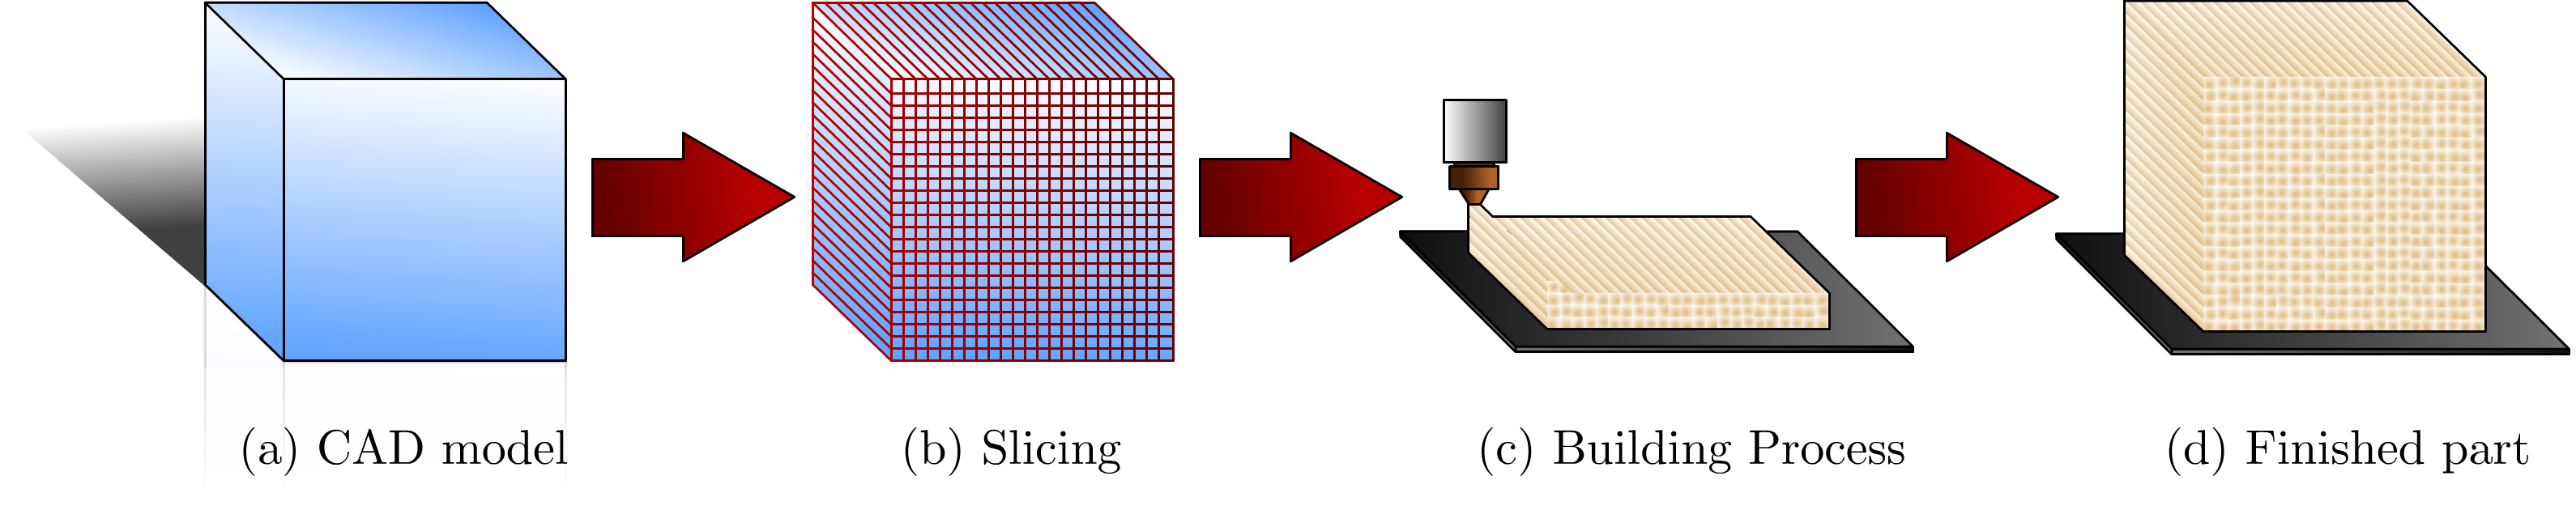
\includegraphics[width=\linewidth]{AM_flowchart_1}
	\caption{Process flow of AM} \label{fig:AM_flow}
\end{figure}

While all AM technologies operate on the same basic process flow described above, the number of different techniques and materials is staggering: ranging from processes that use paper and binder, all the way through metal-based, laser tracing technologies, it is easy to see that the spectrum of AM is broad.
\subsection{Fused Filament Fabrication}
%Nomenclature introduced in this chapter:
\nomenclature[A]{SLA}{Stereolithography}% 
\nomenclature[A]{SLS}{Selective Laser Sintering}%
\end{document}